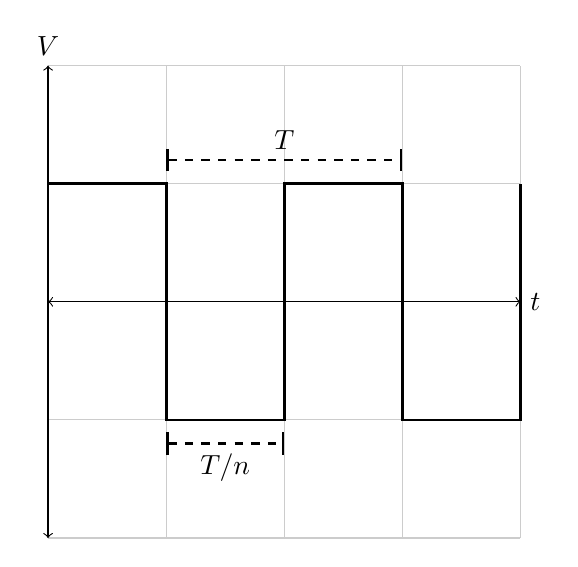
\begin{tikzpicture}[scale=1.5]

    \draw[thin,gray!40] (0,0) grid (4,4);
    
    
    \draw[<->] (0,2)--(4,2) node[right] {$t$};
    \draw[<->] (0,0)--(0,4) node[above]{$V$};

    \draw[line width=1pt,black](0,3)--(1,3)--(1,1)--(2,1)--(2,3)--(3,3)--(3,1)--(4,1)--(4,3);
    \draw[line width=1pt,black,|-|,dashed](1,3.2)--(3,3.2) node[midway,above]{$T$};
    \draw[line width=1pt,black,|-|,dashed](1,0.8)--(2,0.8) node[midway,below]{$T/n$};
\end{tikzpicture}
